\documentclass[12pt]{article}

\usepackage{amsmath}
\usepackage{amssymb}
\usepackage{amsthm}
\usepackage{mathtools}

\usepackage{xcolor}

%\usepackage[textheight=8.5in, margin=1.6in]{geometry}
\usepackage[total={6in,8in}]{geometry}

\usepackage{tikz}
\usepackage{tikz-cd}
\tikzset{
      labl/.style={anchor=south, rotate=90, inner sep=.5mm}
      }
%\usepackage{pgfplots}
\tikzstyle{ball} = [circle,shading=ball, ball color=black,
    minimum size=1mm,inner sep=1.3pt]
%\usetikzlibrary{arrows.meta}
%\tikzset{>={Latex[length=2mm,width=1.5mm]}}

%\usepackage{graphicx}

\usepackage{needspace}  % <-- to prevent bad pagebreak over environment titles
% Use:  \Needspace{3\baselineskip} before opening an environment

\usepackage{enumitem}
\setlist[enumerate]{leftmargin=*}

%\usepackage[colorlinks=true,citecolor=black,linkcolor=black,urlcolor=blue]{hyperref}

\newcommand{\N}{\mathbb{N}}
\newcommand{\Z}{\mathbb{Z}}
\newcommand{\Q}{\mathbb{Q}}
\newcommand{\R}{\mathbb{R}}
\newcommand{\C}{\mathbb{C}}
\newcommand{\T}{\mathbf{T}}
\newcommand{\tL}{\widetilde{L}}
\newcommand{\tF}{\widetilde{F}}
\newcommand{\tH}{\widetilde{H}}
\newcommand{\tD}{\widetilde{D}}
\newcommand{\tb}{\tilde{\beta}}
\newcommand{\sn}{\mathfrak{S}}
\newcommand{\ve}{\varepsilon}
\newcommand{\proj}{\mathbb{P}}
\newcommand{\ips}[2]{\langle{#1}, {#2}\rangle}
\DeclareMathOperator{\tr}{tr}
\DeclareMathOperator{\Span}{\mathrm{Span}}
\DeclareMathOperator{\rk}{\mathrm{rank}}
\DeclareMathOperator{\trace}{\mathrm{tr}}
\DeclareMathOperator{\im}{\mathrm{im}}
\DeclareMathOperator{\Sym}{\mathrm{Sym}}
\DeclareMathOperator{\Hom}{\mathrm{Hom}}
\DeclareMathOperator{\Ext}{\mathrm{Ext}}
\DeclareMathOperator{\cut}{\mathcal{C}}
\DeclareMathOperator{\flow}{\mathcal{F}}
\DeclareMathOperator{\diag}{\mathrm{diag}}
\DeclareMathOperator{\glb}{\mathrm{glb}}
\DeclareMathOperator{\lub}{\mathrm{lub}}
\DeclareMathOperator{\crit}{\mathcal{K}}
\DeclareMathOperator{\skel}{Skel}
\DeclareMathOperator{\cok}{\mathrm{cok}}

\newcommand{\pup}[1]{\partial_{\,\Upsilon,{#1}}}

\newtheorem{theorem}{Theorem}[section]
\newtheorem{lemma}[theorem]{Lemma}
\newtheorem{cor}[theorem]{Corollary}
\newtheorem{prop}[theorem]{Proposition}

\theoremstyle{definition}
\newtheorem{definition}[theorem]{Definition}
\newtheorem{example}[theorem]{Example}
\newtheorem{xca}[theorem]{Exercise}

\theoremstyle{remark}
\newtheorem{remark}[theorem]{Remark}

%\parskip = 0.05in
%\parindent = 0.0in

%\pagestyle{empty}

\begin{document}
\centerline{\sc notes on chip-firing for simplicial complexes}
\bigskip

\section{Forests}
Let~$\Delta$ be a~$d$-dimensional simplicial complex.  Denote its set
of~$i$-faces by~$\Delta_i$, and define~$f_i:=|\Delta_i|$.

\begin{definition}\label{def: spanning forest} 
  A {\em spanning forest of $\Delta$} is a $d$-dimensional subcomplex
  $\Upsilon\subseteq\Delta$ with $\skel_{d-1}(\Upsilon)=\skel_{d-1}(\Delta)$ and
  satisfying the three conditions:
  \begin{enumerate}[leftmargin=*]
    \item\label{sst1}  $\tH_d(\Upsilon)=0$;
    \item\label{sst2}  $\tb_{d-1}(\Upsilon)=\tb_{d-1}(\Delta)$;
    \item\label{sst3}  $f_d(\Upsilon) = f_d(\Delta)-\tb_d(\Delta)$.
  \end{enumerate}
  If $0\le k<d$, a \emph{$k$-dimensional spanning forest} of $\Delta$
  is a~$k$-dimensional spanning forest of the $k$-skeleton
  $\skel_{k}(\Delta)$.  In the case where~$\tb_{d-1}(\Delta)=0$, a~$d$-dimension spanning forest called a
  {\em spanning tree}.  The complex~$\Delta$ is called a {\em forest} if it is a
  spanning forest of itself, i.e., if~$\tH_d(\Delta)=0$.
\end{definition}

\noindent{\bf Remarks.}  Let~$\Upsilon$ be a subcomplex of~$\Delta$ sharing the
same~$(d-1)$-skeleton.
\begin{enumerate}
  \item The condition~$\tH_d(\Upsilon)=0$ is equivalent to the elements of the
    set
    \[
A:=\left\{\pup{d}(f):f\in\Upsilon_d \right\}
    \]
    being linearly independent (over~$\Z$ or, equivalently, over~$\Q$).
  \item Since~$\Upsilon$ and~$\Delta$ have the same~$(d-1)$-skeleton,
    $\partial_{\Delta,d-1}=\pup{d-1}$, and
    hence,~$\tb_{d-1}(\Upsilon)=\tb_{d-1}(\Delta)$ is equivalent
    to~$\rk\im\pup{d}=\rk\im\partial_{\Delta,d}$. 
  \item It follows from the above two remarks that~$\Upsilon$ is a spanning
    forest if and only if~$A$, defined above, is a basis for~$\im\partial_{\Delta,d}$ over~$\Q$,
    i.e, the columns of the matrix~$\partial_{\Delta,d}$ corresponding to
    the~$d$-faces of~$\Upsilon$ are a~$\Q$-basis for the column space
    of~$\partial_{\Delta,d}$.  In particular, spanning forests always exist.
\end{enumerate}

\begin{prop} Any two of the three conditions defining a spanning forest implies
  the remaining condition.
\end{prop}

\begin{definition}  Define the {\em complexity} or {\em forest number} of~$\Delta$ to be
  \[
    \tau:=\tau_d(\Delta):=\sum_{\Upsilon\subseteq\Delta}|\T(\tH_{d-1}(\Upsilon))|^2
  \]
  where the sum is over all ($d$-dimensional) spanning forests of~$\Delta$.
\end{definition}

\begin{prop}~$\tau_d(\Delta)=1$ if and only if~$\Delta$ is a forest.
\end{prop}
\begin{proof} 
  Suppose that~$\tau_d(\Delta)=1$.  Then~$\Delta$ possesses a unique spanning
  forest~$\Upsilon$.  It follows that the set columns of~$\partial_d$ has a unique
  maximal linearly independent subset---those columns corresponding to the faces
  of~$\Upsilon$.  Since the columns of~$\Delta$ are all nonzero, it must be that
  the columns corresponding to~$\Upsilon$ are the only columns,
  i.e.,~$|\Upsilon_d|=|\Delta_d|$, and hence~$\Upsilon=\Delta$.
  
  Conversely, suppose that~$\Delta$ is a forest and
  that~$\Upsilon\subseteq\Delta$ is a spanning forest.  Since~$\tH_d(\Delta)=0$,
  it follows that
  \[
    |\Upsilon_d|=|\Delta_d|-\tb_d(\Delta)=|\Delta_d|.
  \]
  Hence,~$\Upsilon=\Delta$, and~$\tau_d(\Delta)=|\T\tH_{d-1}(\Delta)|^2=1$.
\end{proof}

\begin{definition}  The~{\em $i$-th Laplacian} of~$\Delta$
  is~$L_i:=\partial_{i+1}\circ\partial_{i+1}^t$.  The {\em $i$-th critical
  group} of~$\Delta$ is
  \[
    \crit_i(\Delta):=\ker\partial_i/\im L_i.
  \]
\end{definition}

\begin{theorem}  Suppose that~$\Upsilon$ is an~$i$-dimensional spanning forest
  of~$\Delta$ such that $\tH_{i-1}(\Upsilon)=\tH_{i-1}(\Delta)$.
  Let~$\Theta:=\Delta_i\setminus\Upsilon_i$.  Define the~{\em reduced
  Laplacian}~$\tilde{L}$ of~$\Delta$ with respect to~$\Upsilon$ to be the square submatrix
  of~$L_{i}$ consisting of the rows and columns indexed
  by~$\Theta$.  Then there is an isomorphism
  \[
    \crit_{i}(\Delta)\to\Z\Theta/\im\tilde{L}
  \]
  obtained by setting the faces of~$\Upsilon_{i}$ equal to~$0$.
\end{theorem}
\begin{proof}  Considering the commutative diagram
\begin{center}
\begin{tikzcd}
  \Z\Upsilon_i\arrow[r,"\pup{i}"]\arrow[d]
  &\Z\Upsilon_{i-1}\arrow[r,"\pup{i-1}"]\arrow[d,equal]
  &\Z\Upsilon_{i-2}\arrow[d,equal]\\
  \Z\Delta_i\arrow[r,"\partial_{\Delta,i}"]
  &\Z\Delta_{i-1}\arrow[r,"\partial_{\Delta,i-1}"]
  &\Z\Delta_{i-2}
\end{tikzcd}
\end{center}
  we see
\[
  \im\pup{i}\subseteq\im\partial_{\Delta,i}\subseteq\ker\partial_{\Delta,i-1}=
  \ker\pup{i-1}.
\]
Thus, there is an exact
\[
  0\to\im\partial_{\Delta,i}/\im\pup{i}\to\tH_{i-1}(\Upsilon)\to\tH_{i-1}(\Delta)\to0.
\]
By hypothesis~$\tH_{i-1}(\Upsilon)=\tH_{i-1}(\Delta)$, and hence
\[
  \im\pup{i}=\im\partial_{\Delta,i}.
\]

  We now describe a basis for~$\ker_{\Delta,i}$.  For each~$\theta\in\Theta$,
  since~$\im\pup{i}=\im\partial_{\Delta,i}$, 
  \begin{equation}\label{eqn: coords}
    \partial_{\Delta,i}(\theta)=\sum_{\tau\in\Upsilon_i}a_{\theta}(\tau)\pup{i}(\tau)
  \end{equation}
  for some~$a_{\theta}(\tau)\in\Z$.  Since~$\tH_i(\Upsilon)=0$, the boundary
  mapping~$\pup{i}$ is injective, and thus the coefficients~$a_{\tau,\theta}$ are
  uniquely determined. Define
  \[
    \alpha(\theta):=\sum_{\tau\in\Upsilon_i}a_{\theta}(\tau)\tau
  \]
  and extend linearly to get a mapping~$\alpha:\Z\Theta\to\Z\Upsilon$.
  For each~$\theta\in\Theta$, let
  \[
    \hat{\theta}:=\theta-\alpha(\theta).
  \]
  We claim 
  \[
    \ker\partial_{\Delta,i}
    =\{\hat{\theta}:\theta\in\Theta\}.
  \]
  The~$\hat{\theta}$ are linearly independent elements of the kernel.
  To show they span, suppose that~$\gamma=\sum_{\sigma\in\Delta_i}b_{\sigma}\sigma\in\ker_{\Delta,i}$. 
  Consider
  \[
    \gamma':=\gamma-\sum_{\theta\in\Theta}b_{\sigma}\hat{\sigma}
    =\sum_{\sigma\in\Upsilon_i}b_{\sigma}\sigma+\sum_{\sigma\in\Theta}b_{\sigma}(\sigma-\hat{\sigma})
    =\sum_{\sigma\in\Upsilon_i}b_{\sigma}\sigma+\sum_{\sigma\in\Theta}b_{\sigma}\alpha(\sigma).
  \]
  Then since~$\gamma$ and the~$\hat{\sigma}$ are in~$\ker_{\Delta,i}$, so
is~$\gamma'$.  Further, since each~$\alpha(\sigma)\in\Z\Upsilon_i$, so
  is~$\gamma'$.  But~$\partial_{\Delta,i}$ restricted to~$\Upsilon_i$ is equal
  to~$\partial_{\Upsilon,i}$, which is injective. It follows that
  \[
    \gamma=\sum_{\sigma\in\Delta_i}b_{\sigma}\sigma=\sum_{\sigma\in\Theta}b_{\sigma}\hat{\sigma}.
  \]
  We thus have an isomorphism
  \[
    \pi\colon
    \Z\Theta\xrightarrow{\ \sim\ }\ker\partial_{\Delta,i}
  \]
  determined by~$\sigma\mapsto\hat{\sigma}$ with inverse given by setting
  elements of~$\Upsilon_i$ equal to~$0$:
  \[
    \sum_{\sigma\in\Delta_i}b_{\sigma}\sigma\xmapsto{\quad\ } \sum_{\sigma\in\Theta}b_{\sigma}\sigma.
  \]

  Next, we claim there is a commutative diagram with exact rows
  \begin{center}
    \begin{tikzcd}
      \Z\Theta\arrow[r,"\tilde{L}"]\arrow[d,"\iota"]
      &\Z\Theta\arrow[r]\arrow[d,"\pi","\sim" labl]
      &\cok\tilde{L}\arrow[r]\arrow[d,dashed]
      &0\\
      \Z\Delta_i\arrow[r,"L_i"]
      &\ker\partial_{\Delta,i}\arrow[r]
      &\crit_i(\Delta)\arrow[r]
      &0
    \end{tikzcd}
  \end{center}
  where~$\iota$ is the natural inclusion.  To check commutativity of the square
  on the left, let~$\theta\in\Theta$.  Then
  \[
    L_i\iota(\theta)=\rho+\tilde{L}\theta
  \]
  for some~$\rho\in\Z\Upsilon$.  We then
  have~$\pi^{-1}(\rho+\tilde{L}\theta)=\tilde{L}\theta$.  Hence, there is a
  well-defined vertical mapping on the left.  By the snake lemma, that mapping is
  an isomorphism if and only if
  \[
    \Z\Theta\xrightarrow{\iota}\Z\Delta_i/\ker L_i
  \]
  is surjective.  Therefore, to finish the proof, we must show that for
  all~$\gamma\in\Upsilon_i$, there exists~$\delta\in\Z\Theta$ such
  that~$\gamma+\delta\in\ker L_i$.

  Now~$\ker L_i=\ker
  \partial_{\Delta,i}\partial_{\Delta,i}^t=\ker\partial_{\Delta,i}^t$. To get a
  description of~$\ker_{\Delta,i}^t$, consider the exact sequence
  \[
    \Z\Delta_{i+1}\xrightarrow{\partial_{\Delta,i+1}}\Z\Delta_i\to\cok\partial_{\Delta,i+1}\to0.
  \]
  Applying the left-exact functor~$\Hom(\,\cdot\,,\Z)$, gives the exact sequence
  \begin{equation}\label{eqn: ker}
    \Z\Delta_{i+1}\xleftarrow{\partial_{\Delta,i+1}^t}\Z\Delta_i\leftarrow(\cok\partial_{\Delta,i+1})^*\leftarrow0,
  \end{equation}
  where we have identified each~$\Z\Delta_{j}$ with its dual using dual bases.
  There is an exact sequence,
  \[
    0\to\ker\partial_{\Delta,i}/\im\partial_{\Delta,i+1}\to\Z\Delta_i/\im\partial_{\Delta,i+1}
    \to\Z\Delta_i/\ker\partial_{\Delta,i}\to0,
  \]
  i.e,
  \begin{equation}\label{eqn: cok}
    0\to\tH_i(\Delta)\to\cok\partial_{\Delta,i+1}\to\Z\Delta_i/\ker\partial_{\Delta,i}\to0.
  \end{equation}
  However,
  \[
    \Z\Delta_i/\ker\partial_{\Delta,i}\xrightarrow{\ \sim\ }\im\partial_{\Delta,i}=\im\partial_{\Upsilon,i}\approx\Z\Upsilon
  \]
  since~$\partial_{\Upsilon,i}$ is injective.  Since~$\Z\Upsilon$ is free,
  sequence~\eqref{eqn: cok} splits:
  \[
    \cok\partial_{\Delta,i+1}\approx\tH_i(\Delta)\oplus\Z\Upsilon.
  \]
  Given~$\gamma\in\Upsilon$, let~$\gamma^*$ be the dual function.  Using the
  above isomorphism, we identify~$\gamma^*$ with an
  element of~$(\cok\partial_{\Delta,i+1})^*$.  Using equation~\eqref{eqn:
  coords}, its image in~$\Z\Delta_i$ under the mapping in~\eqref{eqn: ker} is
  \[
    \gamma+\sum_{\theta\in\Theta}a_{\theta}(\gamma)\theta,
  \]
  which by exactness of~$\eqref{eqn: ker}$ is an element
  of~$\ker\partial_{\Delta,i+1}^t$.
  Letting~$\delta:=\sum_{\theta\in\Theta}a_{\theta}(\gamma)\theta$, we
  see~$\gamma+\delta\in\ker\partial_{\Delta,i+1}$, as required.
\end{proof}

\noindent{\bf Question.}  Is there still a mapping between these two groups in
the case~$\tH_{d-1}(\Delta)\neq\tH_{d-1}(\Upsilon)$?

\begin{definition}  Define the {\em cut and flow spaces} and the {\em cut and
  flow lattices} of~$\Delta$ by:
  \begin{align*}
    \mathrm{Cut}(\Delta)&:=\im_{\R}\partial_d^{t}, &\mathrm{Flow}(\Delta)&:=\ker_{\R}\partial_d\\
    \cut(\Delta)&:=\im_{\Z}\partial_d^{t},\qquad
    &\flow(\Delta)&:=\ker_{\Z}\partial_d.
  \end{align*}
  (NOTE: Need to define the cocritical group.)
\end{definition}

\begin{theorem}\label{thm: cut flow sequences}
  There are exact sequences
  \begin{align*}
    0\to\Z^n/(\cut+\flow)\to\cut^{\sharp}/\cut\approx\T(\crit_{d-1}(\Delta))\to\T(\tH_{d-1}(\Delta))\to0\\[8pt]
    0\to\T(\tH_{d-1}(\Delta))\to\Z^n/(\cut+\flow)\to\flow^{\sharp}/\flow\approx\T(\crit^*_{d-1}(\Delta))\to0
  \end{align*}
  Further,~$|\T(\crit_{d-1}(\Delta))|=\tau(\Delta)$.
\end{theorem}

\centerline{\sc old stuff}
\medskip

Fix the standard inner product on~$\R^n$.  If~$\mathcal{L}\subseteq\Z^n$, define
the dual lattice of~$\mathcal{L}$ by
\[
  \mathcal{L}^{\sharp}:=\left\{ v\in\mathcal{L}\otimes\R:\langle
  v,w\rangle\in\Z\ \forall w\in\mathcal{L} \right\}.
\]
\begin{prop} With notation as above, we have
  \begin{enumerate}
    \item $\mathcal{L}^{\sharp}\approx\Hom_{\Z}(\mathcal{L},\Z)$.
    \item $(\mathcal{L}^{\sharp})^{\sharp}=\mathcal{L}$.
  \end{enumerate}
\end{prop}
\begin{proof}
\end{proof}


\begin{prop}\label{prop: AC1}
Suppose that $\Delta$ is a $d$-dimensional simplicial complex. Then~$\Delta$ possesses a simplicial spanning tree if and only if $\tb_{d-1}(\Delta)=0$. We say that such complexes are \emph{acyclic in codimension 1}.
\index{simplicial complex!spanning trees of!and acyclicity}
\end{prop}
\begin{proof}
First suppose that $\Upsilon$ is a spanning tree of $\Delta$. Then $C_d(\Upsilon)\subset C_d(\Delta)$, $C_{d-1}(\Upsilon)=C_{d-1}(\Delta)$, and $\im(\partial_{\Upsilon,d})\subseteq\im(\partial_{\Delta,d})$. It follows that there is a surjection
\[
\tH_{d-1}(\Upsilon)=C_{d-1}(\Upsilon)/\im(\partial_{\Upsilon,d})\twoheadrightarrow 
C_{d-1}(\Delta)/\im(\partial_{\Delta,d})=\tH_{d-1}(\Delta).
\]
Since $\tH_{d-1}(\Upsilon)$ is finite, it follows that $\tH_{d-1}(\Delta)$ is also finite, hence $\tb_{d-1}(\Delta)=~0$.

Now suppose that $\Delta$ is acyclic in codimension 1. To construct a spanning tree, start with $\Upsilon=\Delta$. If $\tH_d(\Upsilon)=0$, then $\Upsilon$ is a spanning tree, and we are done. If not, then there is an integer-linear combination of facets $\sigma_i$ in the kernel of $\partial_d$:
\[
a_1\sigma_1+a_2\sigma_2+\cdots+a_k\sigma_k,
\]
where we assume that $a_1\ne 0$. If we work over the rational numbers, then we may assume $a_1=1$. Still working over the rationals, we see that 
\[
\partial_d(\sigma_1)=-\sum_{i=2}^ka_i\partial_d(\sigma_i).
\]
Hence, if we remove the facet $\sigma_1$ from $\Upsilon$, we obtain a smaller subcomplex $\Upsilon'$ without changing the image of the rational boundary map: $\im(\partial_{\Upsilon,d})=\im(\partial_{\Upsilon',d})$. It follows from rank-nullity that
\[
\tb_d(\Upsilon')=f_d(\Upsilon')-\rk\,\im(\partial_{\Upsilon',d})=f_d(\Upsilon)-1-\rk\,\im(\partial_{\Upsilon,d})
=\tb_d(\Upsilon)-1,
\]
and $\tb_{d-1}(\Upsilon')=\tb_{d-1}(\Upsilon)=0$. Continuing to remove facets in this way, we eventually obtain a spanning tree of $\Delta$.
\end{proof}

\begin{cor}\label{cor: AC1} If~$0\leq i\leq d$, then~$\Delta$ has
  an~$i$-dimensional spanning tree if and only if~$\tb_{i-1}(\Delta)=0$.
\end{cor}
\begin{proof} This follows from the previous proposition
  since~$\tb_{i-1}(\skel(\Delta))=\tb_{i-1}(\Delta)$.
\end{proof}

\begin{prop}\label{prop: unique tree} If~$\Delta$ has a unique~$d$-dimensional spanning tree~$\Psi$,
  then~$\Delta=\Psi$.
\end{prop}
\begin{proof}
  To come.
\end{proof}

Let~$0\leq i\leq d$.  The {\em $i$-th tree number} for~$\Delta$ is
\[
  \tau_i:=\tau_i(\Delta):=\sum_{\Psi}|H_{i-1}(\Psi)|^2,
\]
where the sum is over all~$i$-dimensional spanning trees of~$\Delta$.

\begin{cor}\label{cor: tree number}
  $\tau_d(\Delta)=1$ if and only if~$\Delta$ is a tree
  and~$\tH_{d-1}(\Delta)=0$, i.e., if and only
  if~$\tH_d(\Delta)=\tH_{d-1}(\Delta)=0$.
\end{cor}
\begin{proof}
  This follows directly from the definition of~$\tau_d(\Delta)$ and
  Proposition~\ref{prop: unique tree}.
\end{proof}

Suppose that $\tb_{i-1}(\Delta)=0$.  It follows that~$\Delta$ has an
$i$-dimensional spanning tree~$\Upsilon$. Let
\[
  \tD_i:=\Delta_i(\Delta)\setminus \Delta_i(\Upsilon),
\]
the $i$-faces of $\Delta$ not contained in $\Upsilon$, and let $\tL_i$ be the
$i$-Laplacian of~$\Delta$ with the rows and columns corresponding to faces in
$\Delta_i(\Upsilon)$ removed.

\begin{theorem}[Duval, Klivans, Martin]\label{thm: simplicial matrix-tree}
  \leavevmode
\begin{enumerate}[label={\rm (\roman*)}]
  \item\label{thm: smt1}  If $\tH_{i-1}(\Upsilon)=0$, there is an isomorphism
    \[
      \psi\colon\crit_i(\Delta)\to \Z\tD_i/\im(\tL_i),
    \]
    defined by dropping $i$-faces
    of $\Upsilon$:   if
    $c=\sum_{f\in \Delta_i(\Delta)}c_f\cdot f\in\ker\partial_i$ represents an element
    of $\crit_i(\Delta)$, then 
    \[
      \psi(c)=\sum_{f\in\tD_i}c_f\cdot f\ \bmod\im(\tL_i).
  \]
\item\label{thm: smt2} (Simplicial matrix-tree theorem)
  \[
    \tau_{i+1}=\frac{|\tH_{i-1}(\Delta)|^2}{|\tH_{i-1}(\Upsilon)|^2}\,\det(\tL_i).
  \]
\end{enumerate}
\end{theorem}

\section{Degrees}
\begin{definition} Let~$0\leq i\leq d$.  The {\em $i$-th positive kernel}
  for~$\Delta$ is the pointed cone
  \[
    \ker^{+}L_i:=\left\{ D\in \Z \Delta_i: D(\sigma)\geq0\ \text{for all $\sigma\in \Delta_i$}
    \right\}.
  \]
  Fixing an ordered Hilbert basis~$H_i=(h_1,\dots,h_{\ell})$ for
  $\ker^{+}L_i$, define the {\em degree}
  of a chain~$D\in\Z \Delta_i$ by
  \[
    \deg(D):= (D\cdot h_1,\dots, D\cdot h_{\ell})
  \]
  where~$D\cdot h_j:=\sum_{\sigma\in \Delta_i}D(\sigma)h_j(\sigma)$.  
  We say~$d\in\Z^{\ell}$ is a {\em winning degree (in dimension~$i$)} if
  each~$D\in \Z \Delta_i$
  with~$\deg(D)\geq d$ is winnable.
\end{definition}

\begin{prop} The degree of a chain depends only on its linear equivalence
  class. 
\end{prop}
\begin{proof} It suffices to show that every element of~$\im L_i$ has degree
  zero.  If~$\tau\in\ker L_i$ and~$\sigma\in\Z\Delta_i$, 
  \[
    \langle \tau,L_i\sigma\rangle
    =\langle L_i^t\tau,\sigma\rangle
    =\langle L_i\tau,\sigma\rangle
    =0,
  \]
  since~$L_i$ is symmetric.
\end{proof}
\begin{cor}
  If a chain~$D$ is winnable, then~$\deg(D)\geq0$.
\end{cor}
\begin{proof}  If~$D$ is winnable, then~$D\sim E$ for some~$E\geq0$.
  Then~$\deg(D)=\deg(E)$, and since
  each element of the Hilbert basis has nonnegative
  coefficients,~$\deg(E)\geq0$.
\end{proof}
\begin{proof}
  See Jesse Kim's thesis for a ``minimal criminal'' argument using the
  {\em stars},~$\partial_i^t(\sigma)$, of elements~$\sigma\in\Delta_{i-1}$.
\end{proof}
\begin{lemma}  For each~$i$, there is a strictly positive element~$\alpha\in\ker
  L_i$, i.e., such that~$\alpha_j>0$ for all~$j$. 
\end{lemma}
\begin{cor} For each~$i$, the~$\Z$-span of~$\ker^{+}L_i$ is~$\ker L_i$.
Hence, 
\[
  (\ker^{+}L_i)^{\perp}=(\ker L_i)^{\perp}=(\ker\partial_{i+1}^t)^{\perp}.
  \]
\end{cor}
\begin{proof}
  Take a strictly positive element~$\alpha\in\ker L_i$ that is primitive, i.e., such
  that the components of~$\alpha$ are relatively prime.  We can then
  complete~$\left\{ \alpha \right\}$ to a basis~$\left\{ \alpha, \beta_1,\dots,\beta_k\right\}$.
  (To see this, consider the exact sequence
  \[
    0\to \Z\alpha\to\Z^n\to\Z^n/\Z\alpha\to0.
  \]
Since~$\Z^n/\Z\alpha$ is torsion free, so the sequence splits.) Then, for
each nonzero~$N\in\Z$, the set~$\left\{ \alpha,
\beta_1+N\alpha,\dots,\beta_k+N\alpha\right\}$ is still a basis for~$\ker L_i$.
By taking~$N\gg 0$, this basis will consist solely of elements
of~$\ker^{+}L_i$.
\end{proof}

\begin{prop}\label{prop: deg 0 iso} For $0\leq i\leq d$, 
\[
  (\ker L_i)^{\perp}/\im(L_i)\approx \T(\crit_i(\Delta)).
\]
Hence, the group of~$i$-chains of degree~$0$ modulo firing rules is
isomorphic to the torsion part of the~$i$-th critical group
of~$\Delta$.
\end{prop}
\begin{proof} 
  To see that~$\im L_i\subseteq(\ker L_i)^{\perp}$, let~$\sigma\in\Z\Delta_i$
  and~$\tau\in\ker L_i=\ker\partial_{i+1}^t$.  Then
  \[
    \langle \tau,L_i\sigma\rangle
    =\langle \tau,\partial_{i+1}\partial_{i+1}^t\sigma\rangle
    =\langle \partial_{i+1}^t\tau,\partial_{i+1}^t\sigma\rangle
    =\langle 0,\partial_{i+1}^t\sigma\rangle
    =0.
  \]
  We also have~$(\im \partial_i^t)\subseteq\ker\partial_i$.  To see
  this, take~$\sigma\in(\im\partial_i^t)^{\perp}$ and~$\tau\in\Z\Delta_i$.  Then
  \[
    0=\langle \sigma,\partial_i^t\tau\rangle=\langle\partial_\sigma,\tau\rangle.
  \]
  Since~$\tau$ is arbitrary,~$\partial_i\sigma=0$.

  Next, 
  \[
    \im\partial_{i}^t\subseteq\ker\partial_{i+1}^t
    \Rightarrow
   (\ker L_i)^{\perp}=(\ker\partial_{i+1}^t)^{\perp}\subseteq(\im\partial_i^t)^{\perp}\subseteq\ker\partial_i.
  \]
  Hence,
  \[
    (\ker L_i)^{\perp}/\im L_i\subseteq\ker\partial_i/\im L_i=:\crit_i(\Delta).
  \]
  Since~$\dim_{\Q}(\ker L_i)^{\perp}=\dim_{\Q}\im L_i$, the group $(\ker
  L_i)^{\perp}/\im L_i$ is finite, and hence torsion.  So it is a subset
  of~$\T(\crit_i(\Delta))$.  To show the opposite inclusion,
  let~$\sigma\in\ker\partial_i$, and suppose there exists a positive
  integer~$n$ such that~$n\sigma\in\im L_i$.  Say~$n\sigma=L_i\tau$, and
  let~$\nu\in\ker L_i=\ker\partial_{i+1}^t$.  Then
  \[
    n\langle \nu,\sigma\rangle
    =\langle \nu,n\sigma\rangle
    =\langle \nu,L_i\tau\rangle
    =\langle \partial_{i+1}^t\nu,\partial_{i+1}^t\tau\rangle
    =0.
  \]
  Therefore,~$\langle\nu,\sigma\rangle=0$. So each torsion element
  of~$\crit_i(\Delta)$ is an element of~$(\ker L_i)^{\perp}$.
\end{proof}

\begin{prop}\label{prop: degree 0 implies forest} All divisors (cycles of
  codimension~1) of degree~$0$ on~$\Delta$ are winnable if and only
  if~$\tau(\Delta)=1$, i.e., if and only if~$\Delta$ is a forest. 
\end{prop}
\begin{proof}  The divisors of degree~$0$ are~$(\ker L_{d-1})^{\perp}$, and
  hence, by Proposition~\ref{prop: deg 0 iso}, these divisors are winnable if
and only if~$\T(\crit_{d-1})(\Delta)=0$.  The result then follows from
Theorem~\ref{thm: cut flow sequences}.
\end{proof}

\begin{definition}  The {\em positive lattice} is
  \[
    \Lambda(\Delta) = \Span_{\N}\left\{ \partial_{d-1}(e):e\in\Delta_{d-1} \right\}.
  \]
\end{definition}

\begin{lemma} The natural
  surjection~$\crit_i(\Delta)\to\tH_i(\Delta)$ is an isomorphism
  when restricted to the free parts of~$\crit_i(\Delta)$ and~$\tH_i(\Delta)$
  and a surjection when retricted to the torsion parts.
\end{lemma}
\begin{proof} Consider the exact sequence
  \[
    0\to\im\partial_{i+1}/\im L_i\to\crit_i(\Delta)\to\tH_i(\Delta)\to0.
  \]
  We have
  \[
    \im L_i\subseteq\im\partial_{i+1}\subseteq(\ker L_i)^{\perp}.
  \]
  So from Proposition~\ref{prop: deg 0 iso}, it follows that~$\im\partial_{i+1}/\im
  L_i$ is finite.  Tensoring the sequence by~$\Q$ then gives the result about
  the free parts, and since the torsion functor~$\T(\,\cdot,)$ is
  left-exact, there is a surjection for the torsion parts.
\end{proof}

\begin{prop}  Let
  \[
    X:=\left\{ D\in\Z\Delta_{d-1}:\partial_{d-1}(D)\in\Lambda(\Delta) \right\}.
  \] 
  Then every~$D\in X$ is winnable if and only if~~$\Delta$ is a forest, acyclic
  in codimension~$1$, i.e., if and only if $\tH_d(\Delta)=\tH_{d-1}(\Delta)=0$.
\end{prop}
\begin{proof}  Note that~$D\in\Lambda(\Delta)$ if and only if~$D=E+A$ for
  some~$E\geq0$ and~$A\in\ker\partial_{d-1}$.  Thus, the condition
  that every~$D\in\Lambda(\Delta)$ is winnable is equivalent to the condition
  that~$\ker\partial_{d-1}=\im L_{d-1}$, i.e,~$\crit_{d-1}(\Delta)=0$.

  ($\Rightarrow$) Suppose every~$D\in\Lambda(\Delta)$ is winnable so
  that~$\crit_{d-1}(\Delta)=0$.  By Theorem~\ref{thm: cut flow sequences}, we
  have~$|\T(\crit_{d-1})|=\tau_d(\Delta)$.  Thus,~$\tau_d(\Delta)=1$, so
  that~$\Delta$ is a forest, or equivalently,~$\tH_d(\Delta)=0$.  Further, there is a
  surjection~$\crit_{d-1}(\Delta)\twoheadrightarrow\tH_{d-1}(\Delta)$.
  So~$\tH_{d-1}(\Delta)=0$.

  ($\Leftarrow$) Conversely, suppose that~$\tH_{d}(\Delta)=\tH_{d-1}(\Delta)=0$.
  The fact that~$\tH_d(\Delta)=0$ says~$\Delta$ is a forest.  So~$\tau_d(\Delta)=1$, which implies
  that~$\crit_{d-1}(\Delta)$ is free by Theorem~\ref{thm: cut flow sequences}.
  However, the free part of~$\crit_{d-1}(\Delta)$ is the same as the free part
  of~$\tH_{d-1}(\Delta)$.  Therefore,~$\crit_{d-1}(\Delta)=0$.
\end{proof}

\begin{example}
  Consider the simplicial complex~$\Delta$ pictured in Figure~\ref{fig: positive
  lattice}. Since $\tH_2(\Delta)=0$, the complex is a forest, but
  since~$\tH_{1}(\Delta)=\Z\neq0$, it is not a tree.  
  Thus, by Proposition~\ref{prop: degree 0 implies forest}, a divisor is
  winnable if and only if its degree is~$0$.  Order the edges lexicographically.
  Consider a generator for the first
  homology such as 
  \[
    D=(0,1,-1,0,0,1)=\overline{02}+\overline{23}-\overline{03}.
  \]
  The Hilbert basis for the positive kernel is given by the rows of the matrix
  \[
  \left(\begin{array}{rrrrrr}
      0 & 0 & 1 & 0 & 0 & 0 \\
      0 & 0 & 0 & 0 & 1 & 1 \\
      1 & 1 & 0 & 0 & 0 & 0 \\
      0 & 1 & 0 & 1 & 1 & 0
  \end{array}\right).
  \]
  Therefore,~$\deg(D)=(-1,1,1,1)$, so~$D$ is not winnable.
  However,~$\partial_1(D)=0\in\Lambda(\Delta)$.
\end{example}

\begin{figure}[ht] 
  \centering
  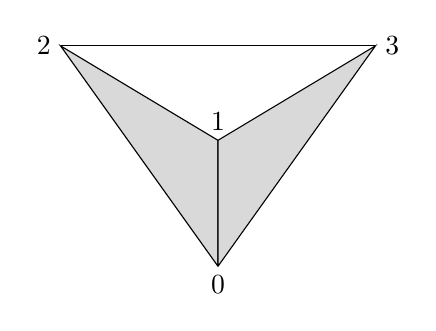
\begin{tikzpicture}[scale=0.8] 
  \draw (0,0) node[below]{$0$} -- (0,2) node[above]{$1$};
  \draw (-2.5,3.5) node[left]{$2$} -- (2.5,3.5) node[right]{$3$};
  \draw[fill=gray!30] (0,0)--(0,2)--(-2.5,3.5)--(0,0);
  \draw[fill=gray!30] (0,0)--(0,2)--(2.5,3.5)--(0,0);
\end{tikzpicture} 
\caption{A hollow tetrahedron with two missing facets.}\label{fig: positive
lattice} 
\end{figure}

\bigskip
\centerline{\sc old stuff}
\medskip

\begin{theorem} If~$\tau_d(\Delta)=1$, then~$0$ is a winning degree in
  dimension~$d-1$. 
\end{theorem}
\begin{proof} Since~$\tau_d(\Delta)=1$, by Proposition~\ref{cor: tree number},
  we have~$\tH_d(\Delta)=\tH_{d-1}(\Delta)=0$.  Thus,~$\partial_d$ is injective,
  and~$\im\partial_d=\ker\partial_{d-1}$.
  The universal coefficient theorem gives an exact sequence
  \[
    0\to\Ext^1(H_{d-1}(\Delta),\Z)\to H^d(\Delta)\to\Hom(H_d(\Delta),\Z)\to0,
  \]
  which implies that~$H^d(\Delta)=0$. We have~$\tH^d(\Delta)=\tH^d(\Delta)$
  for~$d>0$.  In the case where~$d=0$, we have that~$\tau_d(\Delta)=1$ implies
  that~$\Delta$ is a single point,~$\partial_{0}$ is an isomorphism, and thus,
  every~$(d-1)$-cycle is linearly equivalent to~$0$.  So we will assume~$d>0$
  from now on.

  To show~$0$ is a winning degree
  in dimension~$d-1$, we must show~$\crit_{d-1}(\Delta)$ is also torsion-free.
  So let~$\alpha\in\ker\partial_{d-1}$ and suppose there exists an
  integer~$n>0$ such that~$n\alpha\in\im(L_{d-1})$.  So there exists~$\beta\in
  C_{d-1}(\Delta)$ such that
  \[
    n\alpha=L_{d-1}\beta=\partial_d\partial_d^t\beta.
  \]
  Since~$\tH_{d-1}(\Delta)=0$,
  there exists~$\gamma\in C_d(\Delta)$ such that~$\partial_d\gamma=\alpha$.  
  Since~$\partial_d$ is injective,~$n\gamma=\partial_d^t\beta$.
  Since~$\tH^d(\Delta)=C^d(\Delta)/\im\partial_d^t=0$, it follows
  that~$\gamma=\im\partial_d^t$, and hence,~$\alpha\in\im L_{d-1}$, as required.
\end{proof}

\begin{example}
  Figure~\ref{fig: real projective plane} illustrates a~$2$-dimensional
  complex~$P$ which is a triangulation of the real projective plane.  We
  have~$\tH_0(P)=\tH_2(P)=0$, and~$\tH_1(P)\approx\Z/2\Z$.  From the definition
  of the tree number,~$\tau_2(P)=4$, and it follows from the matrix-tree theorem
  that~$\det(\tL_0)=4$ with respect to any~$1$-dimensional spanning tree
  of~$P$.  (There are~$6^4$ such spanning trees since the~$1$-skeleton
  of~$P$ is the completer graph~$K_6$.)  The
  cycle~$C:=\overline{01}+\overline{12}-\overline{02}$ has degree~$(0,0,0,0,0)$ but
  is not winnable.  We have~$\crit_1(P)\approx\Z/2\Z\times\Z/2\Z$, and
  hence~$2C$ is winnable.
\begin{figure}[ht] 
  \centering
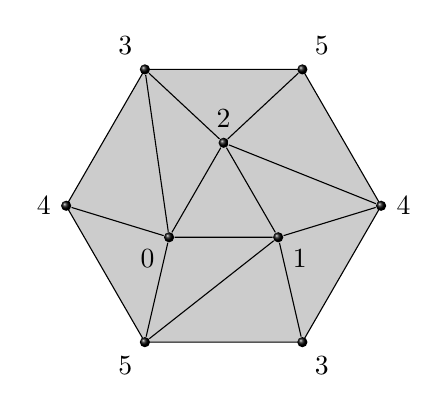
\begin{tikzpicture}
  \def\r{2.0cm}
  \draw[fill=gray!40] ({\r*cos(0*60)},{\r*sin(0*60)})--({\r*cos(1*60)},{\r*sin(1*60)})--({\r*cos(2*60)},{\r*sin(2*60)})--({\r*cos(3*60)},{\r*sin(3*60)})--({\r*cos(4*60)},{\r*sin(4*60)})--({\r*cos(5*60)},{\r*sin(5*60)})--({\r*cos(6*60)},{\r*sin(6*60)});
  
  \draw ({\r*cos(0*60},{\r*sin(0*60)}) node[label=0*60:{$4$},ball] (1) {};
  \draw ({\r*cos(1*60},{\r*sin(1*60)}) node[label=1*60:{$5$},ball] (2) {};
  \draw ({\r*cos(2*60},{\r*sin(2*60)}) node[label=2*60:{$3$},ball] (3) {};
  \draw ({\r*cos(3*60},{\r*sin(3*60)}) node[label=3*60:{$4$},ball] (11) {};
  \draw ({\r*cos(4*60},{\r*sin(4*60)}) node[label=4*60:{$5$},ball] (22) {};
  \draw ({\r*cos(5*60},{\r*sin(5*60)}) node[label=5*60:{$3$},ball] (33) {};

  \def\s{0.8cm}
  \draw ({\s*cos(210},{\s*sin(210)}) node[label=210:{$0$},ball] (4) {};
  \draw ({\s*cos(-30},{\s*sin(-30)}) node[label=-30:{$1$},ball] (5) {};
  \draw ({\s*cos(90},{\s*sin(90)}) node[label=90:{$2$},ball] (6) {};

  \draw (22)--(4);
  \draw (22)--(5)--(33);
  \draw (5)--(1)--(6)--(2);
  \draw (6)--(3)--(4)--(11);
  \draw (6)--(4)--(5)--(6);
\end{tikzpicture}
\caption{A triangulation of the real projective plane, $\R\proj^2$.}\label{fig:
real projective plane} 
\end{figure}
\end{example}

\noindent{\bf Question.}  Can we find an example where~$\tau_d(\Delta)=1$
and~$0$ is not a winning degree in dimension~$d-1$?  The~$2$-dimensional
chessboard complex is an example of a non-tree for which~$0$ is a winning degree
in dimension~$1$.
\bigskip

\noindent{\bf Question.} 

NOTE: The dual of an intersection of cones is the minkowski sum of the duals of
the cones in the intersection.  For example, over the rationals,
\[
  (\ker L_i\cap\mathcal{O}^+)^* = (\ker L_i)^*+(\mathcal{O}^+)^*=(\ker
  L_i)^{\perp}+\mathcal{O}^+.
\]
The expression on the left is the dual of the positive kernel (as a cone),
which is the set of divisors of nonnegative degree.  The expression on the right
is the set of divisors having the same degree as an effective divisor.
\end{document}
